\documentclass[../main.tex]{subfiles}

\begin{document}

\subsection{Robótica social}
La \textbf{robótica social} es una rama de la robótica que se centra en el diseño y desarrollo de robots que pueden interactuar con los humanos de manera efectiva y natural (véase la figura \ref{fig:robotica_social}). 
Estos robots están diseñados para trabajar en entornos sociales, como hogares, hospitales, escuelas y espacios públicos, y su objetivo es facilitar la interacción humano-robot y mejorar la calidad de vida de las personas.
Actualmente, la robótica social está en auge debido a los avances en inteligencia artificial, aprendizaje automático y tecnologías de percepción, lo que ha permitido el desarrollo de robots más sofisticados y capaces de comprender y responder a las necesidades humanas.

\begin{figure}[H]
\centering
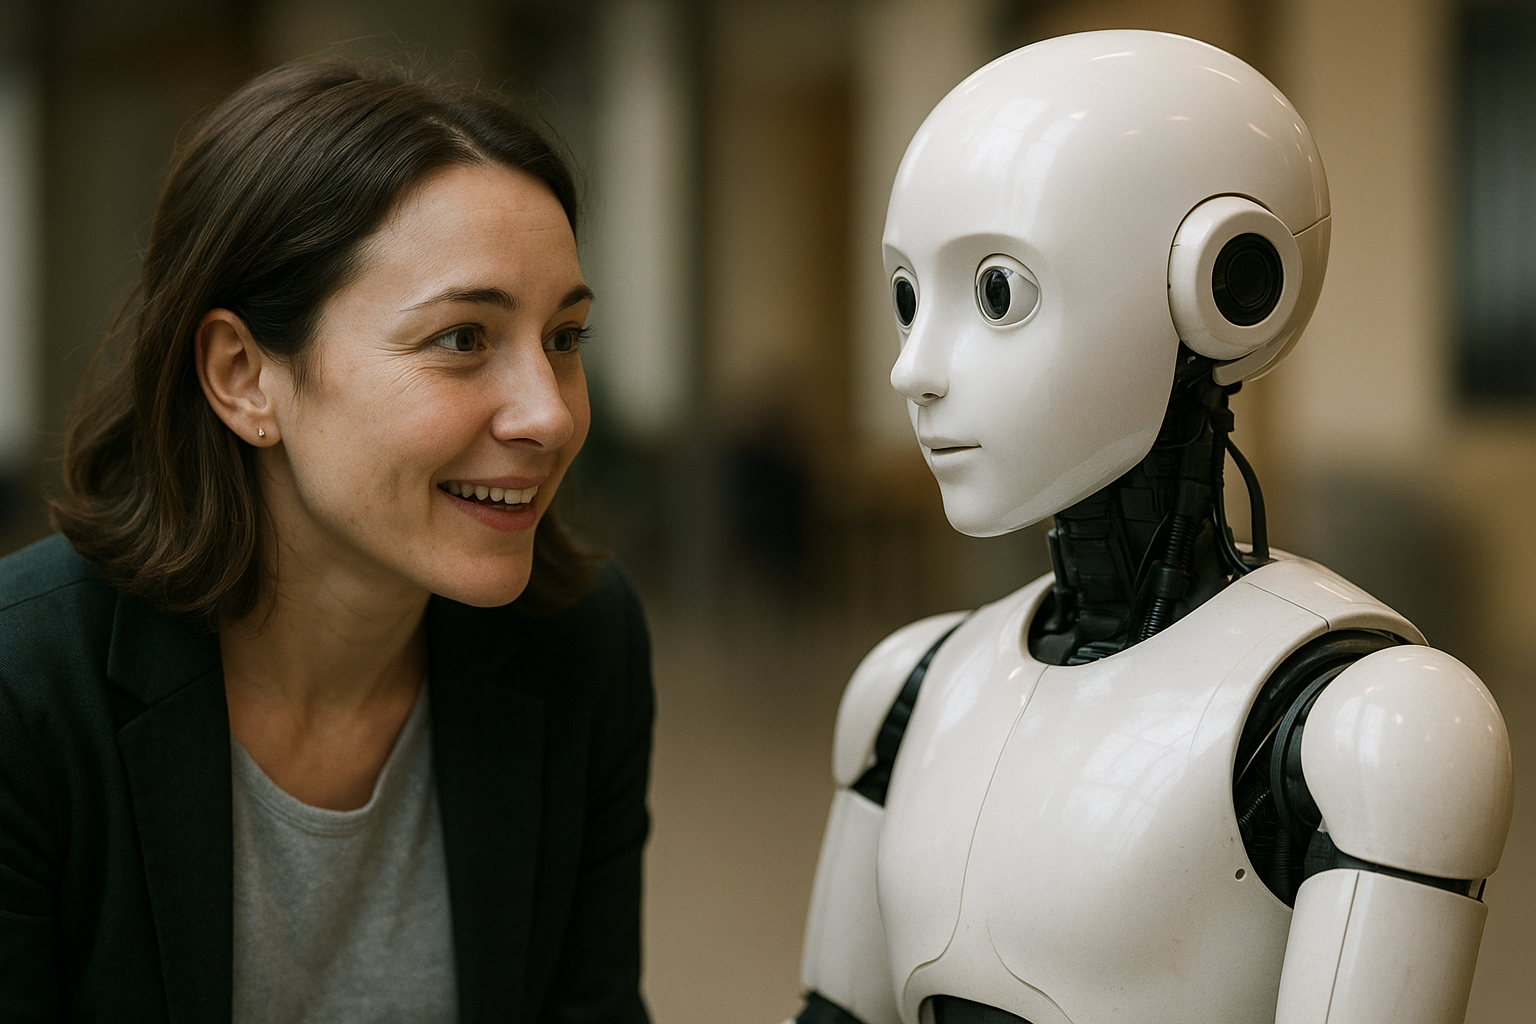
\includegraphics[width=0.75\textwidth]{images/social-robotics.png}
\caption{Ejemplo de un robot social interactuando con un humano}\label{fig:robotica_social}
\end{figure}

Algunos ejemplos de aplicaciones de la robótica social incluyen:
\begin{itemize}
    \item \textbf{Asistentes personales}: Robots diseñados para ayudar a las personas en tareas diarias, como recordatorios, gestión de calendarios y asistencia en el hogar.
    \item \textbf{Educación}: Robots que pueden interactuar con estudiantes y profesores en entornos educativos, facilitando el aprendizaje y la enseñanza.
    \item \textbf{Salud}: Robots que pueden asistir a profesionales de la salud en hospitales y clínicas, proporcionando apoyo a pacientes y personal médico.
    \item \textbf{Entretenimiento}: Robots diseñados para interactuar con personas en entornos de ocio, como museos, parques temáticos y eventos públicos.
    \item \textbf{Compañía}: Robots que pueden proporcionar compañía y apoyo emocional a personas mayores\cite{iglesias2024town} o solas, ayudando a combatir la soledad y el aislamiento social.
\end{itemize}

En el caso de este trabajo, el robot se podría categorizar como un asistente personal, ya que su objetivo consiste en ayudar a los usuarios mediante la realización de distintas tareas.

\subsection{Modelos de Lenguaje a Gran Escala (LLM)}
Los \textbf{modelos de lenguaje a gran escala} son una tecnología que se desarrolló y se popularizó hace pocos años, ganando mucha relevancia casi de forma inmediata
por su gran potencial. Los LLMs comenzaron teniendo la funcionalidad principal de, a partir de unas instrucciones o un \textit{prompt} en lenguaje natural, generar una respuesta
textual razonada y con sentido, pudiendo desde obtener información de un tema concreto, hasta mantener una conversación relacionada con un tema en concreto. 

Actualmente, estos modelos se han ido desarrollando y mejorando de manera exponencial, 
pudiendo no sólo generar texto, sino video e imágenes realistas, y música de cualquier género, todo siguiendo el \textit{prompt} introducido. 

Hoy en día, muchas empresas han decidido entrenar y desarrollar sus propios modelos, existiendo una gran variedad de opciones a elegir. Cada empresa crea modelos
más robustos o más rápidos, los cuales están diseñados para dar una mejor respuesta, ser rápidos o poder ejecutarse en una máquina de menor gama. Algunos modelos son 
\textit{open source} y puedes ejecutarlos en tu propia máquina, en cambio, otros modelos son accesibles mediantes APIs (gratis o de pago).

\begin{itemize}
    \item \textbf{ChatGPT}: Este modelo fue el primer modelo de LLM y el más famoso hasta la fecha, es un modelo de pago para el uso desde APIs desarrollado por la empresa OpenAI.
    \item \textbf{Gemini}: Este modelo tiene versiones gratuitas y de pago para su acceso desde APIs, su desarrollador es Google.
    \item \textbf{Llama}: Este modelo se puede ejecutar desde una máquina propia con un permiso que se le pide a la empresa, en este caso Meta.
    \item \textbf{DeepSeek}: Este modelo es \textit{open source}, es decir, puedes ejecutarla desde un sistema propio sin necesidad de licencia o permiso alguno, y además tiene una API para su acceso
    que también es gratuita.
\end{itemize}

Cada modelo ha sido entrenado con un número de parámetros, que usualmente define su robustez y rapidez a la hora de la ejecución, pero además de esos parámetros, se pueden configurar
otros parámetros como la \textit{temperatura} o el \textit{top\_k} que definen la aleatoriedad (o creatividad) con la que el modelo va a responder a la instrucción. Más creatividad implica
una respuesta menos determinista, por tanto más creativa y similar a una respuesta humana, aunque si el nivel es demasiado alto, puede ser demasiado aleatorio y comenzar a responder mensajes
sin sentido o muy alejados de las instrucciones dadas.

\subsection{Árboles de comportamiento}
Los \textbf{árboles de comportamiento} son una técnica diseñada para tomar decisiones en tiempo real sobre un actor y un escenario concreto. Esta técnica permite que un actor con ciertas
acciones pueda tener cierta lógica e inteligencia sobre las acciones que realiza, sobretodo teniendo en cuenta que las decisiones que se toman varían dependiendo de las circunstancias que puedan
ocurrir durante la ejecución. Esta técnica se utiliza en un gran número de ámbitos, algunos más destacables pueden ser los sistemas de control del robot\cite{ogren2022behavior} o la toma de decisiones de un
Personaje No Jugador dentro del ámbito de los videojuegos. En ambos casos, consigue añadir una inteligencia y un razonamiento sobre las decisiones que se toman, simulando los robots un comportamiento más humano.

A continuación explicaremos el funcionamiento de esta técnica. Los árboles de comportamiento se componen de comportamientos, refiriéndose a los nodos del árbol de decisión. Estos comportamientos pueden ser una acción a ejectuar, o un comportamiento compuesto, los cuales
comentaremos más adelante. Estos comportamientos se ejecutan cada vez que se produce un \textit{tick}, que podemos definir como una iteración por parte del nodo raíz sobre las acciones dentro del árbol. 

Cada comportamiento debe devolver
un \textit{feedback} en cada tick, destacando entre ellos los estados de \textbf{succesful}, \textbf{failure} y \textbf{running}. Su propio nombre indica el estado del comportamiento, por ejemplo, \textbf{succesful} indica que el comportamiento ha terminado correctamente,
\textbf{failure} que ha terminado con fallos y \textbf{running} que aún no ha terminado de ejecutarse. Gracias a estos estados, podemos llevar un control del árbol en tiempo de ejecución. Una vez explicado el contexto de los estados de los comportamientos,
expondremos los distintos tipos de comportamientos y algunos ejemplos:

\begin{itemize}
    \item \textbf{Comportamiento compuesto}: Se refiere a un comportamiento donde se ejecutan varias acciones. Estos comportamientos siguen una lógica para ejecutar las acciones hijas, por ejemplo, un comportamiento
    que debe ejecutar todas sus hijos, y si falla algún hijo falla también el comportamiento (\textit{Comportamiento en secuencia}).
    \item \textbf{Comportamiento simple}: Se refiere a un comportamiento que ejecuta una acción o decisión. Este comportamiento se puede personalizar para las decisiones o acciones que se deseen tomar, proporcionando además
    el estado mencionado anteriormente, que sirve de feedback del sistema. Un ejemplo de este comportamiento puede ser mover el robot a algún sitio.
\end{itemize}

Investigando acerca de los recursos que existen sobre los árboles de comportamiento, se hallan distintas librerías que permiten utilizar esta técnica de forma simple, por ejemplo \textbf{Py Trees} para implementar
estos árboles en el lenguaje \textit{Python} y \textbf{BehaviorTree.CPP} para implementarlos en el lenguaje \textit{C++}.

\end{document}